\begin{comment}
\end{comment}

\chapter{Algorithmes variationnels quantiques}

%-----------------------------------------------------------------------------%

\begin{comment}
\subsection*{Plan}

\begin{enumerate}
    \item Décrire les algorithmes variationels en général
    \item Expliquer les objectifs de ces algorithmes
    \item Expliquer les avantages (exemple: algorithmes à court-terme, qubits bruités)
    \item Expliquer la chronologie avec les QAOA
    \item Expliquer comment est-ce qu'on peut utiliser ceux-ci comme générateur pour l'algorithme JVV.
\end{enumerate}
    
\subsection*{Références}

1. Cerezo, M. et al. Variational quantum algorithms. Nat Rev Phys 3, 625–644 (2021).

2. Bharti, K. et al. Noisy intermediate-scale quantum (NISQ) algorithms. Rev. Mod. Phys. 94, 015004 (2022).
\end{comment}



%-----------------------------------------------------------------------------%

\section{Algorithme quantique d'optimisation approximative}

\subsection*{Plan}

\begin{enumerate}
    \item Expliquer l'histoire et le lien avec le recuit quantique 
\end{enumerate}

\subsection*{Références}

1. Farhi, E., Goldstone, J. and Gutmann, S. A Quantum Approximate Optimization Algorithm. Preprint at https://doi.org/10.48550/arXiv.1411.4028 (2014).

2. Kadowaki, T. and Nishimori, H. Quantum annealing in the transverse Ising model. Phys. Rev. E 58, 5355–5363 (1998).

3. Finnila, A. B., Gomez, M. A., Sebenik, C., Stenson, C. and Doll, J. D. Quantum annealing: A new method for minimizing multidimensional functions. Chemical Physics Letters 219, 343–348 (1994).

4. Farhi, E. et al. A Quantum Adiabatic Evolution Algorithm Applied to Random Instances of an NP-Complete Problem. Science 292, 472–475 (2001).

5. Farhi, E., Goldstone, J., Gutmann, S. and Sipser, M. Quantum Computation by Adiabatic Evolution. Preprint at https://doi.org/10.48550/arXiv.quant-ph/0001106 (2000).

%-----------------------------------------------------------------------------%

\subsection{Description de l'algorithme}

\subsection*{Plan}

\begin{enumerate}
    \item Décrire le \textit{Quantum Approximate Optimization Algorithm}
\end{enumerate}

\subsection*{Références}

1. Farhi, E., Goldstone, J. and Gutmann, S. A Quantum Approximate Optimization Algorithm. Preprint at https://doi.org/10.48550/arXiv.1411.4028 (2014).

%-----------------------------------------------------------------------------%

\subsection{Initialisation des paramètres}

\subsection*{Plan}

\begin{enumerate}
    \item Décrire l'importance d'une bonne initialisation des paramètres (\textit{barren plateau}, non-convexité des paramètres)
    \item Énumérer les principales méthodes
    \item Expliquer l'initialisation aléatoire par grille
    \item Expliquer \textit{TQA}
\end{enumerate}

\subsection*{Références}

1. Bittel, L. and Kliesch, M. Training Variational Quantum Algorithms Is NP-Hard. Phys. Rev. Lett. 127, 120502 (2021).

2. Anschuetz, E. R. and Kiani, B. T. Beyond Barren Plateaus: Quantum Variational Algorithms Are Swamped With Traps. Nat Commun 13, 7760 (2022).

3. Akshay, V., Philathong, H., Morales, M. E. S. and Biamonte, J. D. Reachability Deficits in Quantum Approximate Optimization. Phys. Rev. Lett. 124, 090504 (2020).
    
4. Cain, M., Farhi, E., Gutmann, S., Ranard, D. and Tang, E. The QAOA gets stuck starting from a good classical string. Preprint at https://doi.org/10.48550/arXiv.2207.05089 (2022).

Peut-être une référence de plus qui traite directement des barrens plateau?

%-----------------------------------------------------------------------------%

\subsection{Encodage du problème}

\begin{comment}
\subsection*{Plan}

\begin{enumerate}
    \item Introduire la fonction de coût
    \item Introduire le modèle d'Ising et le modèle QUBO
    \item Décrire la transformation d'Ising pour NAE3SAT et 1in3SAT
    \item Prouver la transformation d'Ising pour NAE3SAT et 1in3SAT
\end{enumerate}

\subsection*{Références}

1. Lucas, A. Ising formulations of many NP problems. Frontiers in Physics 2, (2014).
\end{comment}

\begin{figure}[h]
    \centering
    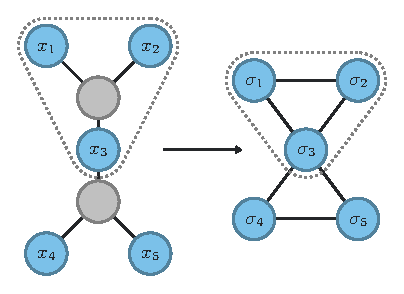
\includegraphics[width=0.5\textwidth]{figures/ising-mapping}
    \caption{}
    \label{fig:...}
\end{figure}


%-----------------------------------------------------------------------------%

\subsection{Choix du forçage}

\subsection*{Plan}

\begin{enumerate}
    \item Expliquer le but du forçage
    \item Expliquer forçage en X
    \item Expliquer le forçage de Grover
    \item Énumérer les forçages populaires
\end{enumerate}

\subsection*{Références}

%-----------------------------------------------------------------------------%

\section{Approche quantique des opérateurs alternants avec forçage de Grover}

\subsection*{Plan}

\begin{enumerate}
    \item Décrire le \textit{Quantum Alternating Operator Ansatz}
    \item Décrire \textit{Grover-Mixer Quantum Alternating Operator Ansatz}
\end{enumerate}

\subsection*{Références}

1. Hadfield, S. et al. From the Quantum Approximate Optimization Algorithm to a Quantum Alternating Operator Ansatz. Algorithms 12, 34 (2019).

2. Bärtschi, A. and Eidenbenz, S. Grover Mixers for QAOA: Shifting Complexity from Mixer Design to State Preparation. in 2020 IEEE International Conference on Quantum Computing and Engineering (QCE) 72–82 (2020). doi:10.1109/QCE49297.2020.00020.

%-----------------------------------------------------------------------------%

\section{Échantillonage et biais}

\subsection*{Plan}

\begin{enumerate}
    \item Expliquer l'importance de l'échantillonnage non-biaisé
    \item Expliquer le problème d'échantillonage associé au recuit quantique
    \item Expliquer le problème d'échantillonage associé à QAOA
    \item Expliquer pourquoi GM-QAOA résout ce problème (ne pas oublier d'expliquer les inconvénients de cette méthode)
\end{enumerate}

\subsection*{Références}

1. Zhang, Z. et al. Grover-QAOA for 3-SAT: Quadratic Speedup, Fair-Sampling, and Parameter Clustering. Preprint at https://doi.org/10.48550/arXiv.2402.02585 (2024).

2. Mandrà, S., Zhu, Z. and Katzgraber, H. G. Exponentially Biased Ground-State Sampling of Quantum Annealing Machines with Transverse-Field Driving Hamiltonians. Phys. Rev. Lett. 118, 070502 (2017).

3. Matsuda, Y., Nishimori, H. and Katzgraber, H. G. Ground-state statistics from annealing algorithms: quantum versus classical approaches. New J. Phys. 11, 073021 (2009).

Plus de sources sur le fair sampling pour QAOA?
